%!TEX root = ../thesis.tex

\cleardoublepage
\chapter{Introduction}

\label{cha:introduction}

%%=========================================
\section{Motivation and Problem Description}
\label{sec:motivation}

One of the aims for the fifth generation of mobile networks (5G) and it's successors will be a greater diversification of the classes of service. As the use cases for these networks evolve, there is a greater need for quality of service (QoS) tailored to each use case. For example, in the Industrial Internet of Things (IIoT) the requirements on latency, jitter, and reliability may be extremely stringent. Supporting these kinds of classes of service can be a challenge for mobile network operators (MNOs) and will require novel approaches to familiar problems, such as backhaul.

As there are more heterogeneous edge deployments and more campus networks, backhaul becomes more challenging, since many sites may not have access to optical fibre, and may be forced into using other solutions such as satellite links, mmWave backhaul, or pre-existing on-site ISP connections. Providing the kind of deterministic quality of service that these sites may require can be a very difficult challenge.

Particularly with the rise of satellite backhaul options, fuelled by the new space race, many remote deployments may choose to integrate satellite backhaul because fibre is infeasible or its rollout is too slow. These connections are usually being added in addition to existing one, and thus network operators may choose to utilize more than one backhaul connection at the same time. Either in order to increase the available bandwidth or to utilize the different qualities of the backhaul links. This bears the question whether multipathing could then be used to provide deterministic backhaul by intelligently selecting on which links to forward packets. This approach bears similarity to multihoming as well as to multi-path routing in Wireless Sensor Networks (WSNs), and can take inspiration from the substantial body of research in these fields which already exists, and which has demonstrated that QoS can be improved by using multiple links or paths simultaneously \cite{akella2003measurement, tao2005improving, habib2007improving, goldenberg2004optimizing, huang2008multiconstrained, akella2008performance}.


%\LTXtable{\textwidth}{tab/scenario1_sensor}

%%=========================================
\section{Goal}
\label{sec:goal}

\begin{figure}[h]
    \centering
        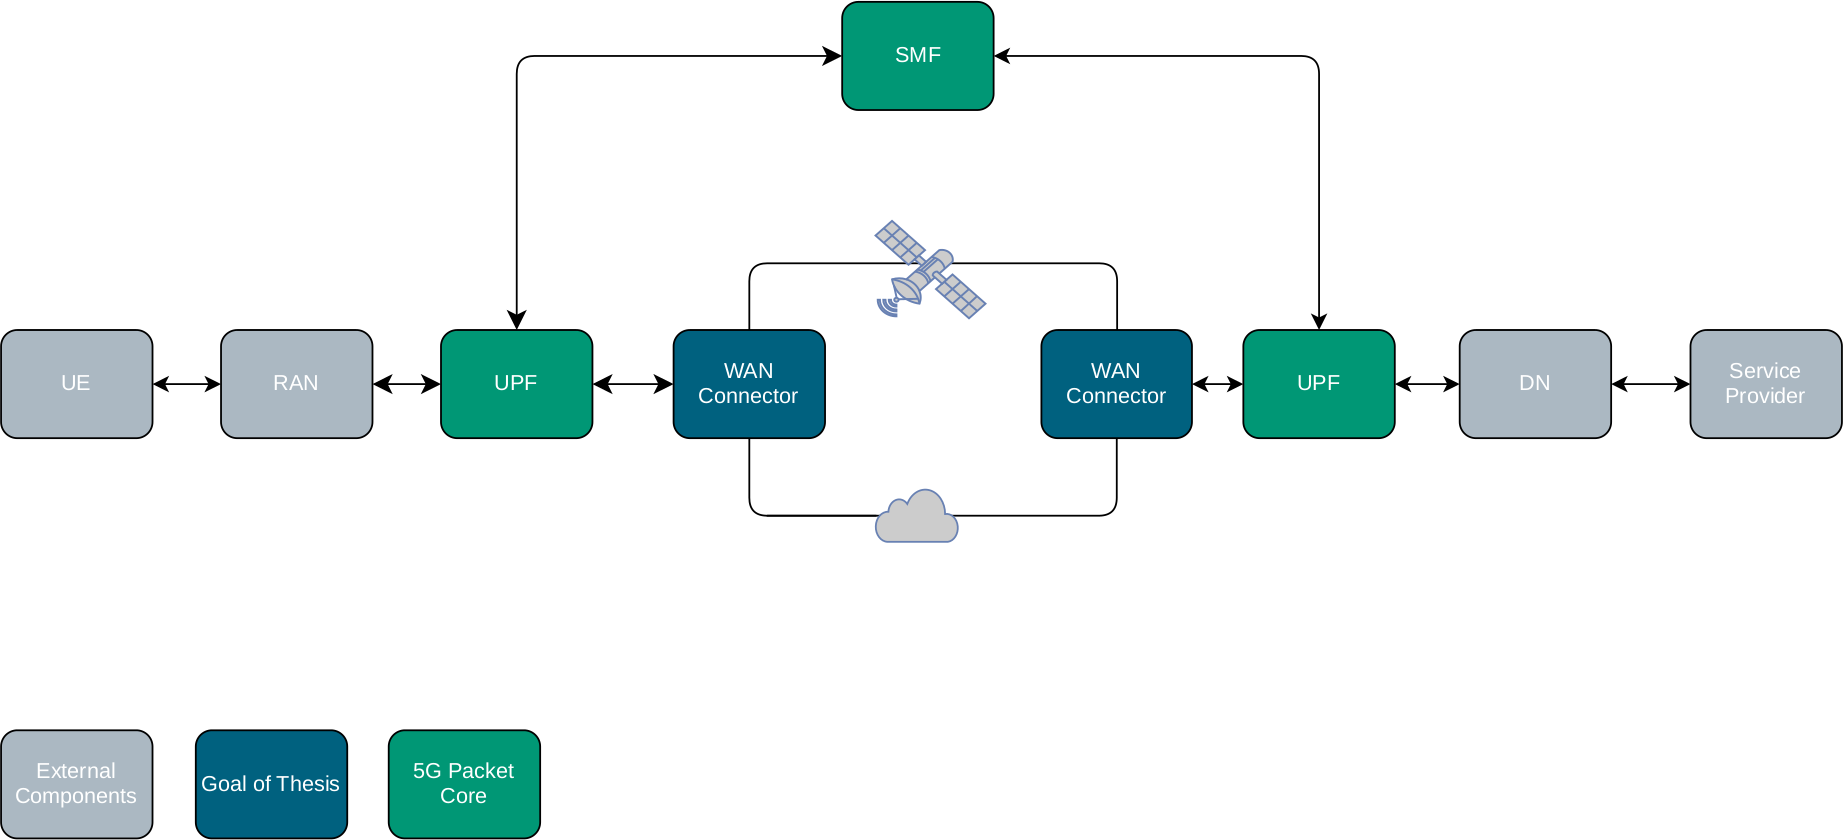
\includegraphics[width=\textwidth]{fig/telco-use-case-2.png}
        \caption{5G Deployment with 2 UPFs}
        \label{fig:telco}
\end{figure}

The goal of this thesis is to design and proivde an implementation of a Wide Area Network (WAN) connector, that can be placed at the ingress and egress point of two or more locations, and utilizes multipathing in order to provide deterministic backhaul between the two sites. The performance of this approach will then be quantitatively analyzed in experiments.

Looking at Figure \ref{fig:telco} we can see how this is envisioned to work. WAN connectors are deployed both in the geographically distributed 5G campus network, which has more than one egress link, and in the core. Then, using the multiple outgoing links, the traffic is backhauled to the other site, while respecting it's QoS requirements. This can be especially beneficial for critical applications (e.g. at industrial sites), which are in locations that do not have access to optical fibre for backhaul.

For a 5G deployment the proposed WAN connector could be deployed in between two User Plane Functions (UPF) , in order to provide deterministic backhaul. The architecture for such a deployment is shown in Figure \ref{fig:telco}. Further, the on-site UPF is not a strict requirement; it is also feasible to connect the RAN directly to the WAN Connector.

%=======================
\section{Structure}

This thesis will follow a simple 5 chapter structure. This section concludes the introduction chapter, what follows will be one chapter to provide both basic background information as well as to highlight the existing literature which is of relevance to the problem statement. Next will be the approach and evaluation chapters, where, respectively, the design of the implementation will be presented and discussed, and then it's performance will be analyzed. The conclusion chapter will review the relevant findings, the successes and failures of the approach, and the possibilities for future research in this area.

%%=========================================

%%% include all citations

% start zotero

%\nocite{kundel_user_2022}
%\nocite{goldenberg_optimizing_nodate}
%\nocite{lange_performance_2015}
%\nocite{tarique_survey_2009}
%\nocite{tschoke_time-sensitive_2021}
%\nocite{ganichev_yamr_2010}
%\nocite{habib_improving_2007}
%\nocite{tao2005improving}
%\nocite{fanglu_guo_experiences_2004}
%\nocite{akella_measurement-based_nodate}
%\nocite{noauthor_zotero_nodate}

% end zotero...


% google scholar

\nocite{tsai2006review}
\nocite{tao2005improving}
\nocite{kundel2022user}
\nocite{goldenberg2004optimizing}
\nocite{lange2015performance}
\nocite{tarique2009survey}
\nocite{tschoke2021time}
\nocite{ganichev2010yamr}
\nocite{habib2007improving}
\nocite{guo2004experiences}
\nocite{akella2003measurement}
\nocite{ergencc2021reliability}
\nocite{tao2004application}
\nocite{alwan2010multi}
\nocite{prados2021asynchronous}
\nocite{zhang2016fundamentals}
\nocite{chen2020collaborative}
\nocite{akella2008performance}
\nocite{andreoli2017mobile}
\nocite{huang2008multiconstrained}
\nocite{capela2014multihoming}
\nocite{sheyibani2012reliable}
\nocite{nguyen2003path}
\nocite{tao2004exploring}
\nocite{bremler2002predicting}
\nocite{zand2012wireless}
\nocite{li2016multipath}
\nocite{finn2019deterministic}
\nocite{finn2019deterministicArch}
\nocite{jaber20165g}
\nocite{xiong2006lightweight}
\nocite{apostolaki2021performance}
\nocite{chebrolu2006bandwidth}
\nocite{stoica1997hierarchical}
\nocite{hoiland2018piece}
\nocite{huang2007wimp}
\nocite{artiga2016terrestrial}
\nocite{rodriguez2004mar}
\nocite{deutschmann2022broadband}
\nocite{murmurhash3}

